% === C01 - Introduccion Bochs ===
% David Alejandro Gonzalez Marquez
% dmarquez@dc.uba.ar / fokerman@gmail.com
% https://github.com/fokerman/Orga2Course

\documentclass[aspectratio=169]{beamer}
% \documentclass[handout]{beamer}

% % % Packages
\usepackage[sfdefault]{AlegreyaSans}
\usepackage{inconsolata}
\usepackage{multicol}
\usepackage{multirow}
\usepackage[spanish]{babel}
\usepackage[utf8]{inputenc}
\usepackage{enumerate}
\usepackage{color}
\usepackage{xcolor}
\usepackage[absolute,overlay]{textpos}
  \setlength{\TPHorizModule}{1mm}
  \setlength{\TPVertModule}{1mm}
\usepackage{framed}
\usepackage{mfirstuc} % para poner en mayusculas la primer letra
\usepackage{xspace} % para crear espacios en comandos 
\usepackage{pbox}
\usepackage{tikz}
\usepackage{mathabx}

% % % Beamer config
\usetheme{Pittsburgh}
\usecolortheme[rgb={1,0.48,0.0}]{structure}
\setbeamercolor{block title}{fg=white,bg=verdeuca}
\xdefinecolor{verdeuca}{rgb}{0.0,0.48,0.54}
\xdefinecolor{naranjauca}{rgb}{1,0.48,0.0}
\setbeamercolor{palette quaternary}{fg=white,bg=verdeuca}
\setbeamertemplate{title page}[default][colsep=-4bp, rounded=true] % remove title shadow
\setbeamertemplate{frametitle}[default][colsep=-2bp, shadow=false] % remove frame title shadow
\setbeamertemplate{navigation symbols}{} % remove navigation symbols
\beamertemplatenavigationsymbolsempty

% % % Colors
\definecolor{AzulClaro}{rgb}{.31,.506,.741}
\definecolor{Gris}{gray}{0.8}
\definecolor{Celeste}{rgb}{.255,.41,.884}
\definecolor{Rojo}{rgb}{1, 0, 0}
\definecolor{a}{rgb}{0.0, 0.53, 0.74}
\definecolor{r}{rgb}{0.89, 0.0, 0.13}
\definecolor{v}{rgb}{0.0, 0.5, 0.0}
\definecolor{y}{rgb}{0.0, 0.5, 0.5}
\definecolor{rojo}{HTML}{F1521B}
\definecolor{verde}{HTML}{80CD29}
\definecolor{amarillo}{HTML}{FABC09}
\definecolor{azul}{HTML}{00ADF1}

% % % Rename
\newcommand{\tab}[0]{\hspace{15pt}}

% % % Blocks
\setbeamercolor{block body}{fg=black, bg=black!10}
\setbeamercolor{block title}{fg=black, bg=black!20}
\setbeamercolor{coloredboxstuffNaranja}{fg=naranjauca,bg=black!10} %% PARA LOS BOX
\setbeamercolor{coloredboxstuffVerde}{fg=verdeuca,bg=black!10} %% PARA LOS BOX

% % % Start

\title{\Huge Introducción a Bochs y el Bootloader}
\subtitle{Programación de Sistemas Operativos}
      
\author{David Alejandro González Márquez}
\institute{Departamento de Computación\\
Facultad de Ciencias Exactas y Naturales\\
Universidad de Buenos Aires}
\date{}

\begin{document}

\frame[plain]{\titlepage}

\begin{frame}[plain]
    \begin{textblock}{55}(10,5)
    \vspace{-0.4cm}
    \begin{center}
    \uncover<2->{\normalsize Programación a nivel de Usuario }
    \end{center}
    \uncover<1->{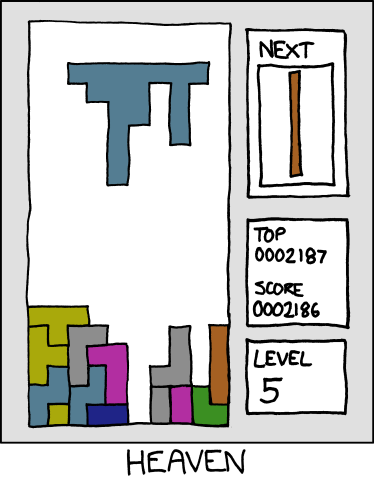
\includegraphics[scale=0.45]{img/heaven.png} }
    \end{textblock}
    \begin{textblock}{60}(88,5)
    \vspace{-0.4cm}
    \uncover<3->{
    \begin{center}
    \normalsize {\normalsize Programación de Sistemas Operativos }
    \end{center}
    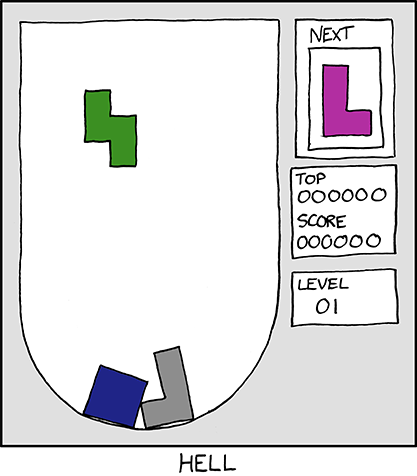
\includegraphics[scale=0.45]{img/hell.png}
    }
    \end{textblock}
    \begin{textblock}{55}(3,85)
    \scriptsize
    \texttt{Fuente: https://xkcd.com/}
    \end{textblock}
\end{frame}

\begin{frame}[plain]
    \begin{textblock}{100}(0,0)
    \uncover<1->{
\includegraphics[scale=0.46]{img/thanos.jpg}}
    \end{textblock}
    \begin{textblock}{100}(0,0)
    \uncover<2->{\includegraphics[scale=0.61]{img/thanos-layer2.pdf}}
    \end{textblock}
    \begin{textblock}{55}(3,85)
    \scriptsize
    \textcolor{white}{\texttt{Fuente: Marvel Comics}}
    \end{textblock}
\end{frame}

\begin{frame}
    \frametitle{Agenda}
    \begin{itemize}\setlength\itemsep{2em}
     \item[-] Introducción a Bochs y su debugger
     \item[-] Funcionamiento y responsabilidades del Bootloader
     \item[-] Comandos para compilar y enlazar código de sistemas
    \end{itemize}
\end{frame}

\begin{frame}
    \frametitle{¿Porque usar bochs?}
    El procesador posee intrucciones que \textbf{no} se pueden usar a nivel de usuario. \\
    \vspace{0.3cm}
    \pause
    Si queremos acceder a estos mecanismos debemos estar en lugar del \textbf{sistema operativo}.
    \vspace{0.6cm}
    \begin{itemize}
    \item<3->[-] Utilizar instrucciones de nivel privilegiado
    \vspace{0.3cm}
    \item<4->[-] Ver estructuras del procesador
    \vspace{0.3cm}
    \item<5->[-] Cambiar modos del procesador
    \vspace{0.3cm}
    \item<6->[-] Acceder a los mecanismos de manejo de memoria
    \vspace{0.3cm}
    \item<7->[-] Controlar interrupciones
    \end{itemize}
\end{frame}

\begin{frame}[t]
    \frametitle{bochs: una Virtual Machine con Debugger}
    \begin{textblock}{140}(10,16)
    Un debugger como \texttt{GDB} es un \textcolor{naranjauca}{proceso} más
    \hspace{0.3cm} {\Large $\Rightarrow$} \hspace{0.3cm}
    No puede monitorear el \textbf{Sistema Operativo}
    \end{textblock}    
    \begin{textblock}{100}(30,25)
    \uncover<2->{\includegraphics[scale=0.65]{img/bochsdbg-layer1.pdf}}
    \end{textblock}
    \begin{textblock}{100}(30,25)
    \uncover<3->{\includegraphics[scale=0.65]{img/bochsdbg-layer2.pdf}}
    \end{textblock}
    \begin{textblock}{100}(30,25)
    \uncover<3->{\includegraphics[scale=0.65]{img/bochsdbg-layer3.pdf}}
    \begin{center}
    \uncover<3->{\Large Bochs + Debugger}
    \end{center}
    \end{textblock}
    \begin{textblock}{135}(10,75)
    \begin{center}
    \uncover<4->{\Large Necesitamos un debugger \textcolor{naranjauca}{\textbf{en}} la Virtual Machine.}
    \end{center}
    \end{textblock}
\end{frame}

\begin{frame}
    \frametitle{Problemas del bochs}
    Es un simulador de una computadora por esto nos permite correr \textbf{instrucción por instrucción}.\\
    \vspace{0.2cm}
    \textbf{Pero} su versión oficial no esta compilada con esta posibilidad.
    \vspace{0.4cm}
    \pause
    \begin{itemize}
    \setlength\itemsep{1em}
    \item[-] bajar de: \small \textbf{\texttt{https://sourceforge.net/projects/bochs/files/bochs/2.6.9/}} \\
    \normalsize el archivo: \small \textbf{\texttt{bochs-2.6.9.tar.gz}}
    \pause
    \item[-] \normalsize descomprimir: \small \textbf{\texttt{tar -xvvzf bochs-2.6.9.tar.gz}}
    \pause
    \item[-] \normalsize en la carpeta descomprimida hacer:\\
    \vspace{0.1cm}
    \begin{itemize}
    \setlength\itemsep{0.5em}
    \item[\texttt{\$}] \small \texttt{./configure --enable-debugger --enable-disasm --disable-docbook\\ 
    --enable-readline LDFLAGS={\char"0D}-pthread{\char"0D}  --prefix=/home/\textcolor{red}{$<usuario>$}/bochs/}
    \item[\texttt{\$}] \small \texttt{make}
    \item[\texttt{\$}] \small \texttt{make install}
    \end{itemize}
    \end{itemize}
\end{frame}

\begin{frame}
    \frametitle{Bonus para instalación}
    Paquetes que pueden faltar instalar:\\
    \vspace{0.3cm}
    \begin{itemize}
    \setlength\itemsep{0.5em}
    \item[\texttt{\$}] \small \texttt{sudo apt-get install xorg-dev}
    \item[\texttt{\$}] \small \texttt{sudo apt-get install libx11-dev}
    \item[\texttt{\$}] \small \texttt{sudo apt-get install libxrandr-dev}
    \item[\texttt{\$}] \small \texttt{sudo apt-get install libgtk2.0-dev}
    \end{itemize}
    \vspace{0.5cm}
    \pause
    Paquete adicional:\\
    \vspace{0.3cm}
    \small Permite tener un buffer de la consola de últimos comandos ejecutados. (aka ``flechitas'')
    \begin{itemize}
    \setlength\itemsep{0.5em}
    \item[\texttt{\$}] \small \texttt{sudo apt-get install libreadline-dev}
    \end{itemize}
\end{frame}

\begin{frame}
    \frametitle{Atajos útiles}
    \textcolor{naranjauca}{Saltar el primer breakpoint y cargar sin menu}\\
    \begin{itemize}
    \item[-] Crear un archivo de nombre \texttt{bochsdbg} con el contenido:
    \begin{itemize}
        \item[] \small \texttt{continue}
    \end{itemize}
    \vspace{0.2cm}
    \item[-] Cargar el bochs usando:
    \begin{itemize}
        \item[\texttt{\$}] \small \texttt{bochs -q -rc bochsdbg}
    \end{itemize}
    \end{itemize}
    \vspace{0.4cm}
    \pause
    \textcolor{naranjauca}{Usar bochs desde cualquier path}\\
    \begin{itemize}
    \item[-] Agregar en el archivo \texttt{/home/\textcolor{red}{$<usuario>$}/.bashrc}:
    \begin{itemize}
        \item[] \small \texttt{ export PATH+=":/home/\textcolor{red}{$<usuario>$}/bochs/bin/" }
    \end{itemize}
    \vspace{0.2cm}
    \item[-] Cargar cambios en la consola actual:
    \begin{itemize}
        \item[\texttt{\$}] \small \texttt{source \textasciitilde/.bashrc }
    \end{itemize}
    \end{itemize}
\end{frame}

\begin{frame}[fragile]
\frametitle{Configuraciones útiles}
    \textcolor{naranjauca}{Activar log de eventos}\\
    \begin{itemize}
    \item[-] Descomentar la siguiente línea del bochsrc:\\
    \begin{itemize}
    \item[] \small \texttt{\#log: bochs.log}
    \end{itemize}
    \item[-] Comentar la siguiente: \\
    \begin{itemize}
    \item[] \small \texttt{log: /dev/null}
    \end{itemize}
    \item[-] Para generar logs de todos los eventos reemplazar:\\
    \begin{itemize}
    \item[] \small \texttt{debug: action=ignore $\longrightarrow$ debug: action=report}
    \end{itemize}
    \small El tamaño del archivo resultante puede ser muy grande ya que registra todos los eventos.
    \end{itemize}
    \vspace{0.2cm}
    \pause
    \textcolor{naranjauca}{Activar GUI del debugger}\\
    \begin{itemize}
    \item[-] Descomentar la siguiente línea del bochsrc: \\
    \begin{itemize}
    \item[] \small \texttt{\#display\_library: x, options="gui\_debug" \# use GTK debugger gui}
    \end{itemize}
    \end{itemize}
\end{frame}

\begin{frame}[fragile]
    \frametitle{Bochs: Config file}
    Para una imagen de linux de ejemplo:
    \small \texttt{http://bochs.sourceforge.net/diskimages.html}
    \scriptsize
    \begin{block}{bochsrc}
    \vspace{-0.3cm}
    \begin{verbatim}
    megs: 32
    romimage: file=$BXSHARE/BIOS-bochs-latest
    vgaromimage: file=$BXSHARE/VGABIOS-lgpl-latest
    vga: extension=vbe
    floppya: 1_44=a.img, status=inserted
    floppyb: 1_44=b.img, status=inserted
    ata0-master: type=disk, path=boot.img, cylinders=900, heads=15, spt=17
    boot: c
    log: bochsout.txt
    mouse: enabled=0
    clock: sync=slowdown
    vga_update_interval: 150000
    display_library: x, options="gui_debug" # use GTK debugger gui
    # This enables the "magic breakpoint" feature when using the debugger.
    # The instruction XCHG BX, BX causes Bochs to enter the debugger mode.
    magic_break: enabled=1
    \end{verbatim}
    \vspace{-0.5cm}
    \end{block}
\end{frame}

\begin{frame}
    \Huge Debugger
\end{frame}

\begin{frame}
    \frametitle{Ejecución: Next y Step}
    \normalsize
    \vspace{0.5cm}
    \begin{itemize}
    \item[-] s $|$ step $|$ stepi [count] \\
    \textcolor{verdeuca}{ejecuta [count] instrucciones} %execute \#count instructions (default is one instruction)
    \vspace{0.2cm}
    \item[-] n $|$ next $|$ p \\
    \textcolor{verdeuca}{Ejecuta instrucciones sin entrar a las subrutinas} %execute instruction stepping over subroutines
    \vspace{0.2cm}
    \item[-] c $|$ cont $|$ continue \\
    \textcolor{verdeuca}{Continua la ejecución} %continue executing
    \vspace{0.2cm}
    \item[-] q $|$ quit $|$ exit \\
    \textcolor{verdeuca}{Sale del debugger y del emulador} %quit debugger and emulator execution
    \vspace{0.2cm}
    \item[-] Ctrl-C \\
    \textcolor{verdeuca}{Detiene la ejecución y retorna al promt} %stop execution, and return to command line prompt
    \end{itemize}
\end{frame}

\begin{frame}[fragile]
    \frametitle{Registros de propósito general}
    \begin{itemize}
    \item[-] r $|$ reg $|$ regs $|$ registers\\
    \textcolor{verdeuca}{Lista los registros del CPU y sus contenidos} %list of CPU registers and their contents
    \end{itemize}
    \small
    \begin{verbatim}
    <bochs:12> registers
    eax: 0x00000000 0
    ecx: 0x00000000 0
    edx: 0x00000543 1347
    ebx: 0x00000000 0
    esp: 0x00000000 0
    ebp: 0x00000000 0
    esi: 0x00000000 0
    edi: 0x00000000 0
    eip: 0x0000e05d
    eflags 0x00000046
    id vip vif ac vm rf nt IOPL=0 of df if tf sf ZF af PF cf
    \end{verbatim}
\end{frame}

\begin{frame}[fragile]
\frametitle{Memory Dump}
    \begin{itemize}
    \item[-] x  /nuf [addr]\\ \textcolor{verdeuca}{Muestra el contenido de la dirección [addr]} %examine memory at linear address
    \vspace{0.2cm}
    \item[-] xp /nuf [addr]\\ \textcolor{verdeuca}{Muestra el contenido de la dirección física [addr]; %examine memory at physical address
            nuf es número que indica cuantos valores se mostrarán, %nuf is a sequence of numbers (how much values to display)
            seguido de uno o más de los indicadores de formato.%and one or more of the [mxduotcsibhwg] format specificators:
            }\\
            \vspace{0.3cm}
            \begin{tabular}{p{2cm}p{2cm}p{2cm}}
            x : hex    & d : decimal & u : sin signo \\
            o : octal  & t : binario & c : char \\
            s : ascii  & i : instrucción & \\
            \end{tabular}\\
            \vspace{0.3cm}
         \textcolor{verdeuca}{y de tamaño}\\
         \vspace{0.3cm}
            \begin{tabular}{p{2cm}p{3cm}p{4cm}}
            b : byte &  h : word = half-word &  w : doubleword = word \\
            \end{tabular}
    \end{itemize}
\end{frame}

\begin{frame}
\frametitle{Memory Disassemble}
    \begin{itemize}
        \item[-]  u $|$ disasm $|$ disassemble [count] [start] [end]\\
        \textcolor{verdeuca}{Desensambla intrucciones desde la dirección lineal [start] hasta [end] exclusive.}%disassemble instructions for given linear address, inclusive of start, exclusive of end.  \\
        \vspace{0.2cm}
        \item[-]  u $|$ disasm $|$ disassemble switch-mode\\
        \textcolor{verdeuca}{Selecciona la sintaxis Intel o AT\&T de asembler.}%switch between Intel and AT\&T disassembler syntax
        \vspace{0.2cm}
        \item[-]  u $|$ disasm $|$ disassemble size = n\\
        \textcolor{verdeuca}{Setea el tamaño del segmento a desensamblar.}%tell debugger what segment size [16\ 32\ 64] to use
    \end{itemize}
\end{frame}

\begin{frame}
\frametitle{Breakpoints}
    \begin{itemize}
    \item[-]  p $|$ pb $|$ break $|$ pbreak [addr] \hspace{0.5cm}
    \textcolor{verdeuca}{Crea un breakpoint en la dirección física [addr]} %set a physical address instruction breakpoint
    \vspace{0.2cm}
    \item[-]  vb $|$ vbreak [seg:offset] \hspace{0.5cm}
    \textcolor{verdeuca}{Crea un breakpoint en la dirección virtual [addr]} %set a virtual address instruction breakpoint
    \vspace{0.2cm}
    \item[-]  lb $|$ lbreak [addr] \hspace{0.5cm}
    \textcolor{verdeuca}{Crea un breakpoint en la dirección lineal [addr]} %set a linear address instruction breakpoint
    \vspace{0.2cm}
    \item[-]  d $|$ del $|$ delete [n] \hspace{0.5cm}
    \textcolor{verdeuca}{Borra el breakpoint número [n]} %delete a breakpoint
    \vspace{0.2cm}
    \item[-]  bpe [n] \hspace{0.5cm}
    \textcolor{verdeuca}{Activa el breakpoint número [n]} %enable a breakpoint
    \vspace{0.2cm}
    \item[-]  bpd [n] \hspace{0.5cm}
    \textcolor{verdeuca}{Desactiva el breakpoint número [n]} %disable a breakpoint
    \end{itemize}
\end{frame}

\begin{frame}
\frametitle{Watchs}
    \begin{itemize}
    \item[-] watch \hspace{0.5cm}
    \textcolor{verdeuca}{Muestra el estado actual de los watchs} %print current watch point status
    \vspace{0.2cm}
    \item[-] watch stop \hspace{0.5cm}
    \textcolor{verdeuca}{Detiene la simulación cuando un watch es encontrado} %stop simulation when a watchpoint is encountred
    \vspace{0.2cm}
    \item[-] watch continue \hspace{0.5cm}
    \textcolor{verdeuca}{No detiene la simulación si un wath es encontrado} %do not stop the simulation when watch point is encountred
    \vspace{0.2cm}
    \item[-] watch r $|$ read [addr] \hspace{0.5cm}
    \textcolor{verdeuca}{Agrega un watch de lectura en la dirección física [addr]} %insert a read watch point at physical address addr
    \vspace{0.2cm}
    \item[-] watch w $|$ write [addr] \hspace{0.5cm}
    \textcolor{verdeuca}{Agrega un watch de escritura en la dirección física [addr]} %insert a write watch point at physical address add
    \end{itemize}
\end{frame}

\begin{frame}
\frametitle{Infos}
    \begin{itemize}
    \item[-] info break \hspace{0.5cm}
    \textcolor{verdeuca}{Muestra los Breakpoint creados} %show information about current breakpoint status
    \vspace{0.2cm}
    \item[-] info eflags \hspace{0.5cm}
    \textcolor{verdeuca}{Muestra el registro EEFLAGS} %show decoded EFLAGS register
    \vspace{0.2cm}
    \item[-] info idt \hspace{0.5cm}
    \textcolor{verdeuca}{Muestra el descriptor de interrupciones (idt)} %show interrupt descriptor table
    \vspace{0.2cm}
    \item[-] info ivt \hspace{0.5cm}
    \textcolor{verdeuca}{Muestra la tabla de vectores de interrupción} %show interrupt vector table
    \vspace{0.2cm}
    \item[-] info gdt \hspace{0.5cm}
    \textcolor{verdeuca}{Muestra la tabla global de descriptores (gdt)} %show global descriptor table
    \vspace{0.2cm}
    \item[-] info tss \hspace{0.5cm}
    \textcolor{verdeuca}{Muestra el segmento de estado de tarea actual (tss)} %show current task state segment
    \vspace{0.2cm}
    \item[-] info tab \hspace{0.5cm}
    \textcolor{verdeuca}{Muestra la tabla de paginas} %show page tables
    \end{itemize}
\end{frame}

\begin{frame}[fragile]
\frametitle{Registros de Segmento}
    \begin{itemize}
        \item[-] sreg \hspace{0.5cm}
    \textcolor{verdeuca}{Muestra los registros de segmento} %show segment registers
    \end{itemize}
    \small{
    \begin{verbatim}
    <bochs:5> sreg
    cs:s=0xf000, dh=0xff0093ff, dl=0x0000ffff, valid=7
    ds:s=0x0000, dh=0x00009300, dl=0x0000ffff, valid=7
    ss:s=0x0000, dh=0x00009300, dl=0x0000ffff, valid=7
    es:s=0x0000, dh=0x00009300, dl=0x0000ffff, valid=7
    fs:s=0x0000, dh=0x00009300, dl=0x0000ffff, valid=7
    gs:s=0x0000, dh=0x00009300, dl=0x0000ffff, valid=7
    ldtr:s=0x0000, dh=0x00008200, dl=0x0000ffff, valid=1
    tr:s=0x0000, dh=0x00008b00, dl=0x0000ffff, valid=1
    gdtr:base=0x00000000, limit=0xffff
    idtr:base=0x00000000, limit=0xffff
    \end{verbatim}
    }
\end{frame}

\begin{frame}[fragile]
\frametitle{Registros de Control}
    \begin{itemize}
        \item[-] creg \hspace{0.5cm}
    \textcolor{verdeuca}{Muestra los registros de control} %show control registers
    \end{itemize}
    \small
    \begin{verbatim}
    <bochs:10> creg
    CR0=0x60000010: pg CD NW ac wp ne ET ts em mp pe
    CR2=page fault laddr=0x00000000
    CR3=0x00000000
        PCD=page-level cache disable=0
        PWT=page-level writes transparent=0
    CR4=0x00000000: osxsave smx vmx osxmmexcpt osfxsr pce pge mce pae pse de tsd pvi vme
    \end{verbatim}
\end{frame}

\begin{frame}[fragile]
    \frametitle{Magic Breakpoint}
    \begin{itemize}
    \item[-] xchg bx, bx \hspace{0.5cm}
    \textcolor{verdeuca}{Magic breakpoint}
    \end{itemize}
    Esta instrucción detiene el flujo del programa y nos devuelve al prompt de bochs.
    \pause
    \begin{center}
    
\includegraphics[scale=2]{img/magic.png}
    \end{center}
    \begin{textblock}{55}(3,85)
    \scriptsize
    \uncover<2->{\texttt{Fuente: Shia LaBeouf `Magic' meme.}}
    \end{textblock}
\end{frame}

\begin{frame}
    \frametitle{Más información}
    \begin{itemize}
    \item[-] \textcolor{verdeuca}{Manual:}\\ \texttt{http://bochs.sourceforge.net/doc/docbook/user/}
    \vspace{0.2cm}
    \item[-] \textcolor{verdeuca}{Información complementaria:}\\ \texttt{http://wiki.osdev.org/Bochs}
    \vspace{0.2cm}
    \item[-] \textcolor{verdeuca}{Imagenes de discos:}\\ \texttt{http://bochs.sourceforge.net/diskimages.html}
    \end{itemize}
\end{frame}

\begin{frame}
    \Huge Bootloader
\end{frame}

\begin{frame}
    \frametitle{Inicio - Pasos de Boot}
    \begin{textblock}{100}(18,16)
    \only<1->{\includegraphics[scale=0.4]{img/Boot_Steps-layer1.pdf}}
    \end{textblock}
    \begin{textblock}{100}(18,16)
    \only<2->{\includegraphics[scale=0.4]{img/Boot_Steps-layer2.pdf}}
    \end{textblock}
    \begin{textblock}{100}(18,16)
    \only<3->{\includegraphics[scale=0.4]{img/Boot_Steps-layer3.pdf}}
    \end{textblock}
    \begin{textblock}{100}(18,16)
    \only<4->{\includegraphics[scale=0.4]{img/Boot_Steps-layer4.pdf}}
    \end{textblock}
    \begin{textblock}{100}(18,16)
    \only<5->{\includegraphics[scale=0.4]{img/Boot_Steps-layer5.pdf}}
    \end{textblock}
\end{frame}

\begin{frame}[fragile]
\frametitle{Resumen}
    \begin{itemize}
    \item[-] Cuando una computadora arranca solo existe el \texttt{BIOS} (Basic Input/Output system).
    \item[-] El proceso de booteo comienza ejecutando el código del \texttt{BIOS}, ubicado en la posición \texttt{0xFFFF0}, en modo real.
    \item[-] El \texttt{BIOS} tiene código en ROM que realiza la inicialización (por ejemplo, la placa de video) y una verificación inicial de la máquina: POST (Power on self-test).
    \item[-] Luego busca algún dispositivo de booteo: Disco Rígido, Floppy, USB, etc...
    \item[-] Una vez localizado el dispositivo de arranque, carga el primer sector de $512$ bytes (CDROM $2048$ bytes) en la posición de memoria \texttt{0x07C00} y salta a esa dirección.
    \item[-] Ahora la imagen de arranque es la encargada de cargar el kernel y luego pasarle el control.
    \item[-] Para que una imagen sea de arranque debe ocupar exactamente 512 bytes (excepto en el CDROM), y estar firmada en los últimos dos bytes con \texttt{0x55AA}.
    \item[-] Una imagen de linux de ejemplo: \texttt{http://bochs.sourceforge.net/diskimages.html}
    \end{itemize}
\end{frame}

\begin{frame}[fragile]
    \frametitle{Ejemplo en Bochs}
    \scriptsize
    \begin{verbatim}
    ------------------------------
    Bochs Configuration: Main Menu
    ------------------------------
    This is the Bochs Configuration Interface, where you can describe the
    machine that you want to simulate.  Bochs has already searched for a
    configuration file (typically called bochsrc.txt) and loaded it if it
    could be found.  When you are satisfied with the configuration, go
    ahead and start the simulation.

    You can also start bochs with the -q option to skip these menus.

    1. Restore factory default configuration
    2. Read options from...
    3. Edit options
    4. Save options to...
    5. Restore the Bochs state from...
    6. Begin simulation
    7. Quit now

    Please choose one: [6]
    \end{verbatim}
\end{frame}

\begin{frame}
\frametitle{Ejemplo en Bochs}
    \begin{itemize}
        \item[-] \textcolor{verdeuca}{Creamos un breakpoint en la posición de memoria física donde comenzará a ser cargado el bootloader} \\
        \vspace{0.2cm}
        \texttt{<bochs:1> break 0x07C00} \\
        \vspace{0.7cm}
        \pause
        \item[-] \textcolor{verdeuca}{Leemos la posición de memoria donde debería estar la firma del bootloader una vez que sea cargado en memoria principal} \\
        \vspace{0.2cm}
        \texttt{<bochs:2> x/1x 0x07C00+510} \\
        \texttt{[bochs]:} \\
        \texttt{0x00007dfe <bogus+       0>:	0x00000000} \\
    \end{itemize}
\end{frame}

\begin{frame}
\frametitle{Ejemplo en Bochs}
    \begin{itemize}
        \item[-] \textcolor{verdeuca}{Continuamos la ejecución, hasta que llegamos al breakpoint} \\
        \vspace{0.2cm}
        \texttt{<bochs:3> c} \\
        \texttt{(0) Breakpoint 1, 0x00007c00 in ?? ()} \\
        \texttt{Next at t=49462126} \\
        \texttt{(0) [0x00007c00] 0000:7c00 (unk. ctxt): cli   ; fa} \\
        \pause
        \vspace{0.7cm}
        \item[-] \textcolor{verdeuca}{Nuevamente, podemos leer y notar que el BIOS cargo los 512bytes pertenecientes al bootloader, primer sector de la unidad} \\
        \vspace{0.2cm}
        \texttt{<bochs:4>  x/1x 0x07C00+510} \\
        \texttt{[bochs]:} \\
        \texttt{0x00007dfe <bogus+       0>:	0x0000aa55} \\
    \end{itemize}
\end{frame}

\begin{frame}[t]
    \frametitle{Bootloader - Pasos para indicar}
    \begin{textblock}{100}(12,12)
    \only<1->{\includegraphics[scale=0.56]{img/BootLoader_Steps-layer1.pdf}}
    \end{textblock}
    \begin{textblock}{100}(12,12)
    \only<2->{\includegraphics[scale=0.56]{img/BootLoader_Steps-layer2.pdf}}
    \end{textblock}
    \begin{textblock}{100}(12,12)
    \only<3->{\includegraphics[scale=0.56]{img/BootLoader_Steps-layer3.pdf}}
    \end{textblock}
    \begin{textblock}{100}(12,12)
    \only<4->{\includegraphics[scale=0.56]{img/BootLoader_Steps-layer4.pdf}}
    \end{textblock}
    \begin{textblock}{100}(12,12)
    \only<5->{\includegraphics[scale=0.56]{img/BootLoader_Steps-layer5.pdf}}
    \end{textblock}
\end{frame}

\begin{frame}
    \frametitle{EL Bootloader de Orga2}
    \begin{textblock}{100}(18,13)
    \only<1->{\includegraphics[scale=0.53]{img/BootLoaderOrga2_Steps-layer1.pdf}}
    \end{textblock}
    \begin{textblock}{100}(18,13)
    \only<2->{\includegraphics[scale=0.53]{img/BootLoaderOrga2_Steps-layer2.pdf}}
    \end{textblock}
    \begin{textblock}{100}(18,13)
    \only<3->{\includegraphics[scale=0.53]{img/BootLoaderOrga2_Steps-layer3.pdf}}
    \end{textblock}
    \begin{textblock}{100}(18,13)
    \only<4->{\includegraphics[scale=0.53]{img/BootLoaderOrga2_Steps-layer4.pdf}}
    \end{textblock}
    \begin{textblock}{100}(18,13)
    \only<5->{\includegraphics[scale=0.53]{img/BootLoaderOrga2_Steps-layer5.pdf}}
    \end{textblock}
    \begin{textblock}{100}(18,13)
    \only<6->{\includegraphics[scale=0.53]{img/BootLoaderOrga2_Steps-layer6.pdf}}
    \end{textblock}
    \begin{textblock}{100}(18,13)
    \only<7->{\includegraphics[scale=0.53]{img/BootLoaderOrga2_Steps-layer7.pdf}}
    \end{textblock}
\end{frame}

\begin{frame}
\frametitle{Compilando y Enlazando}
\begin{center}
\begin{itemize}
    \setlength\itemsep{1em}
\item[-] Un compilador construye un programa de forma que pueda correr sobre un \textbf{sistema operativo} determinado
\pause
\item[-] Para resolver direcciones, toma una \textbf{dirección de inicio}, por ejemplo \texttt{0x00000000}
\pause
\item[-] Cada etiqueta se traduce a una dirección contando \textbf{bytes} desde la dirección de inicio
\pause
\item[-] Los \textbf{destinos} de saltos o llamadas a funciones se debe conocer en tiempo de enlazado
\pause
 \vspace{0.2cm}
\item[-] \large \textcolor{naranjauca}{¿Y si no estamos en un sistema operativo?}\\ \vspace{0.2cm} Ej: el archivo \texttt{KERNEL.BIN} se carga en la dirección \texttt{0x1200}
\end{itemize}
\end{center}
\end{frame}

\begin{frame}
    \frametitle{Compilando y Enlazando}
    \begin{textblock}{100}(8,13)
    \only<1->{\includegraphics[scale=0.44]{img/Compilar_origen-layer1.pdf}}
    \end{textblock}
    \begin{textblock}{100}(8,13)
    \only<2->{\includegraphics[scale=0.44]{img/Compilar_origen-layer2.pdf}}
    \end{textblock}
    \begin{textblock}{100}(8,13)
    \only<3->{\includegraphics[scale=0.44]{img/Compilar_origen-layer3.pdf}}
    \end{textblock}
    \begin{textblock}{100}(8,13)
    \only<4->{\includegraphics[scale=0.44]{img/Compilar_origen-layer4.pdf}}
    \end{textblock}
    \begin{textblock}{100}(8,13)
    \only<5->{\includegraphics[scale=0.44]{img/Compilar_origen-layer5.pdf}}
    \end{textblock}
    \begin{textblock}{100}(8,13)
    \only<6->{\includegraphics[scale=0.44]{img/Compilar_origen-layer6.pdf}}
    \end{textblock}
    \begin{textblock}{100}(8,13)
    \only<7->{\includegraphics[scale=0.44]{img/Compilar_origen-layer7.pdf}}
    \end{textblock}
    \begin{textblock}{100}(8,13)
    \only<8->{\includegraphics[scale=0.44]{img/Compilar_origen-layer8.pdf}}
    \end{textblock}
\end{frame}

\begin{frame}
    \frametitle{Compilando y Enlazando}
    \textbf{Indicar la dirección de origen}\\
    \vspace{0.5cm}
    Hay 2 formas de hacerlo, según como se compile:
    \vspace{0.5cm}
    \pause
    \begin{itemize}
    \setlength\itemsep{1.8em}
    \item[-] De \textbf{ensamblador a binario}, usamos la directiva \texttt{ORG} al inicio del \texttt{archivo.asm} para indicar la direccion de origen\\
    \begin{center}
    \texttt{ORG 0x1200}
    \pause
    \end{center}
    \item[-] De \textbf{ensamblador a elf}, usamos el parámetro \texttt{-Ttext} en el linker\\
    \begin{center}
    \texttt{-Ttext 0x1200}
    \end{center}
    \end{itemize}
\end{frame}

\begin{frame}
    \frametitle{Compilando y Enlazando}
    \textbf{Compilación de ensamblador a binario}\\
    \vspace{0.5cm}
    \begin{itemize}
    \setlength\itemsep{2em}
    \item[-] \textcolor{verdeuca}{Ensamblado:}
    \begin{center}
    \texttt{nasm -fbin archivo.asm -o archivo.bin}
    \end{center}
    \item[-] \textcolor{verdeuca}{Consideraciones:}
    \vspace{0.2cm}
    \begin{itemize}
     \item[$\cdot$] Todo el código ejecutable tiene que estar incluido (No hay bibliotecas)
     \item[$\cdot$] Se ejecuta tal cual se escribió, no hay entry point.
    \end{itemize}
    \end{itemize}
\end{frame}

\begin{frame}
    \frametitle{Compilando y Enlazando}
    \textbf{Compilación de C en formato elf32 y linkeo}\\
    \vspace{0.2cm}
    \begin{itemize}
    \setlength\itemsep{2em}
    \item[-] \textcolor{verdeuca}{Compilación:}\\
    \texttt{gcc -m32 -fno-zero-initialized-in-bss -fno-stack-protector -ffreestanding -c -o archivo.elf archivo.c}
    \item[-] \textcolor{verdeuca}{Linkeo:}\\
    \texttt{ld -static -m elf i386 -nostdlib -N -b elf32-i386 -e start\\ -Ttext 0x1200 -o archivo.elf archivo.o}
    \item[-] \textcolor{verdeuca}{Lo convertimos en binario:}\\
    \texttt{objcopy -S -O binary archivo.elf archivo.bin}
    \end{itemize}
\end{frame}

\begin{frame}
    \frametitle{Compilando y Enlazando}
    \textbf{Compilación de assembly en formato elf32 y linkeo}\\
    \vspace{0.1cm}
    \begin{itemize}
    \setlength\itemsep{1.7em}
    \item[-] \textcolor{verdeuca}{Compilación:}\\
    \texttt{nasm -felf32 archivo.asm -o archivo.o}
    \item[-] \textcolor{verdeuca}{Linkeo:}\\
    \texttt{ld -static -m elf i386 --oformat binary -b elf32-i386 -e start\\ -Ttext 0x1200 archivo.o -o archivo.bin}
    \item[-] \textcolor{verdeuca}{Consideraciones:}
    \begin{itemize}
     \item[$\cdot$] OJO código de 32 bits (en modo protegido)
     \item[$\cdot$] Se pueden usar biblotecas. No se respeta el entry point.
     \item[$\cdot$] El parámetro Ttext da el orígen de la sección .text.
     \item[$\cdot$] Si usan el Bootloader de Orga 2, deben usar 0x1200 como origen de la sección .text.
    \end{itemize}
    \end{itemize}
\end{frame}

\begin{frame}
    \frametitle{Compilando y Enlazando}
    \textbf{Compilación de un bootloader y creacion de diskette}\\
    \vspace{0.2cm}
    \begin{itemize}
    \setlength\itemsep{1.7em}
    \item[-] \textcolor{verdeuca}{Creamos un diskette vacio:}\\
    \texttt{dd bs=512 count=2880 if=/dev/zero of=diskette.img}
    \item[-] \textcolor{verdeuca}{Formateamos la imagen en FAT12:}\\
    \texttt{sudo mkfs.msdos -F 12 diskette.img -n ETIQUETA}
    \item[-] \textcolor{verdeuca}{Escribimos en el sector de booteo:}\\
    \texttt{dd if=bootloader.bin of=diskette.img count=1 seek=0 conv=notrunc}
    \item[-] \textcolor{verdeuca}{Copiado del KERNEL.BIN dentro del diskette}\\
    \texttt{mcopy -i diskette.img kernel.bin ::/}
    \end{itemize}
\end{frame}

\begin{frame}[fragile]
    \frametitle{Bibliografía: Fuentes y material adicional}
    \begin{itemize}
    \item Convenciones de llamados a función en x86: \\
    \url{https://en.wikipedia.org/wiki/X86_calling_conventions}
    \item Notas sobre System V ABI: \\
    \url{https://wiki.osdev.org/System_V_ABI}
    \item Documentación de NASM: \\
    \url{https://nasm.us/doc/}
    \item Artículo sobre el flag \texttt{-pie}: \\
    \url{https://eklitzke.org/position-independent-executables}
    \item Documentación de System V ABI: \\
    \url{https://uclibc.org/docs/psABI-x86_64.pdf}
    \item Manuales de Intel: \\
    \url{https://software.intel.com/en-us/articles/intel-sdm}
    \end{itemize}
\end{frame}

\begin{frame}[plain]
\begin{center}
\vspace{2cm}
\huge ¡Gracias!\\
\vspace{2cm}
\normalsize Recuerden leer los comentarios al final de \\ este video por aclaraciones o fe de erratas.
\end{center}
\end{frame}

\end{document}
